
\renewcommand{\arraystretch}{2}
\renewcommand{\figurename}{Figure}
\chapter{Literature Analysis and State of Art}
\label{chapter:literarure}

\newenvironment{literature}
{\quote\itshape}
{\endquote}

\begin{literature}
This chapter delves into a comprehensive analysis of the current state of art in weapon detection and closed-circuit television (\ac{cctv}) systems. The discussion begins with an overview of the general context in Section 2.1, laying the groundwork for a more detailed examination of weapon detection technologies and \ac{cctv} systems. Section 2.2 delves into object detection, reviewing key algorithms and techniques. Section 2.3 focuses on related research, including methodologies, \ac{cctv} setup, and weapon detection analysis. It concludes with a comprehensive examination of datasets and architectural methods in weapon detection research.
\end{literature}

\section{Context}
\subsection{Weapons}
The Cambridge Dictionary\footnote{https://dictionary.cambridge.org/dictionary/english/weapon} defines a weapon as "any object used in fighting or war, such as a gun, bomb, knife, etc.". This definition suggests that a weapon encompasses any tool or instrument intended to inflict damage or harm, whether on living beings, structures, or systems. Weapons have diverse applications, ranging from hunting and self-defense to warfare. However, their fundamental purpose remains unchanged: they amplify the user's ability to exert force, in either an offensive or defensive capacity.

Weapons can be categorized based on various criteria, including their range, mechanism, or intended use. However, this study will primarily focus on two categories: firearms and melee weapons.

Melee weapons are close-combat instruments that require the user to be in direct proximity to their target, like swords, daggers, maces, and clubs.

Firearms are a subset of ranged weapons that discharge projectiles powered by rapidly expanding high-pressure gas from chemical reactions. They can be further categorized into:
\begin{itemize}
    \item Handguns: Small, handheld firearms like pistols and revolvers.
    \item Rifles: Designed for accuracy, rifles have a longer barrel and are often used in situations requiring precision.
    \item Shotguns: These fire shells that contain multiple pellets, making them effective at close range.
    \item Automatic and Semi-Automatic: Automatic firearms continuously fire bullets as long as the trigger is pressed, while semi-automatics require a trigger pull for each shot.
\end{itemize}

\begin{figure}[h]
    \centering
    \begin{minipage}{0.45\textwidth}
        \centering
        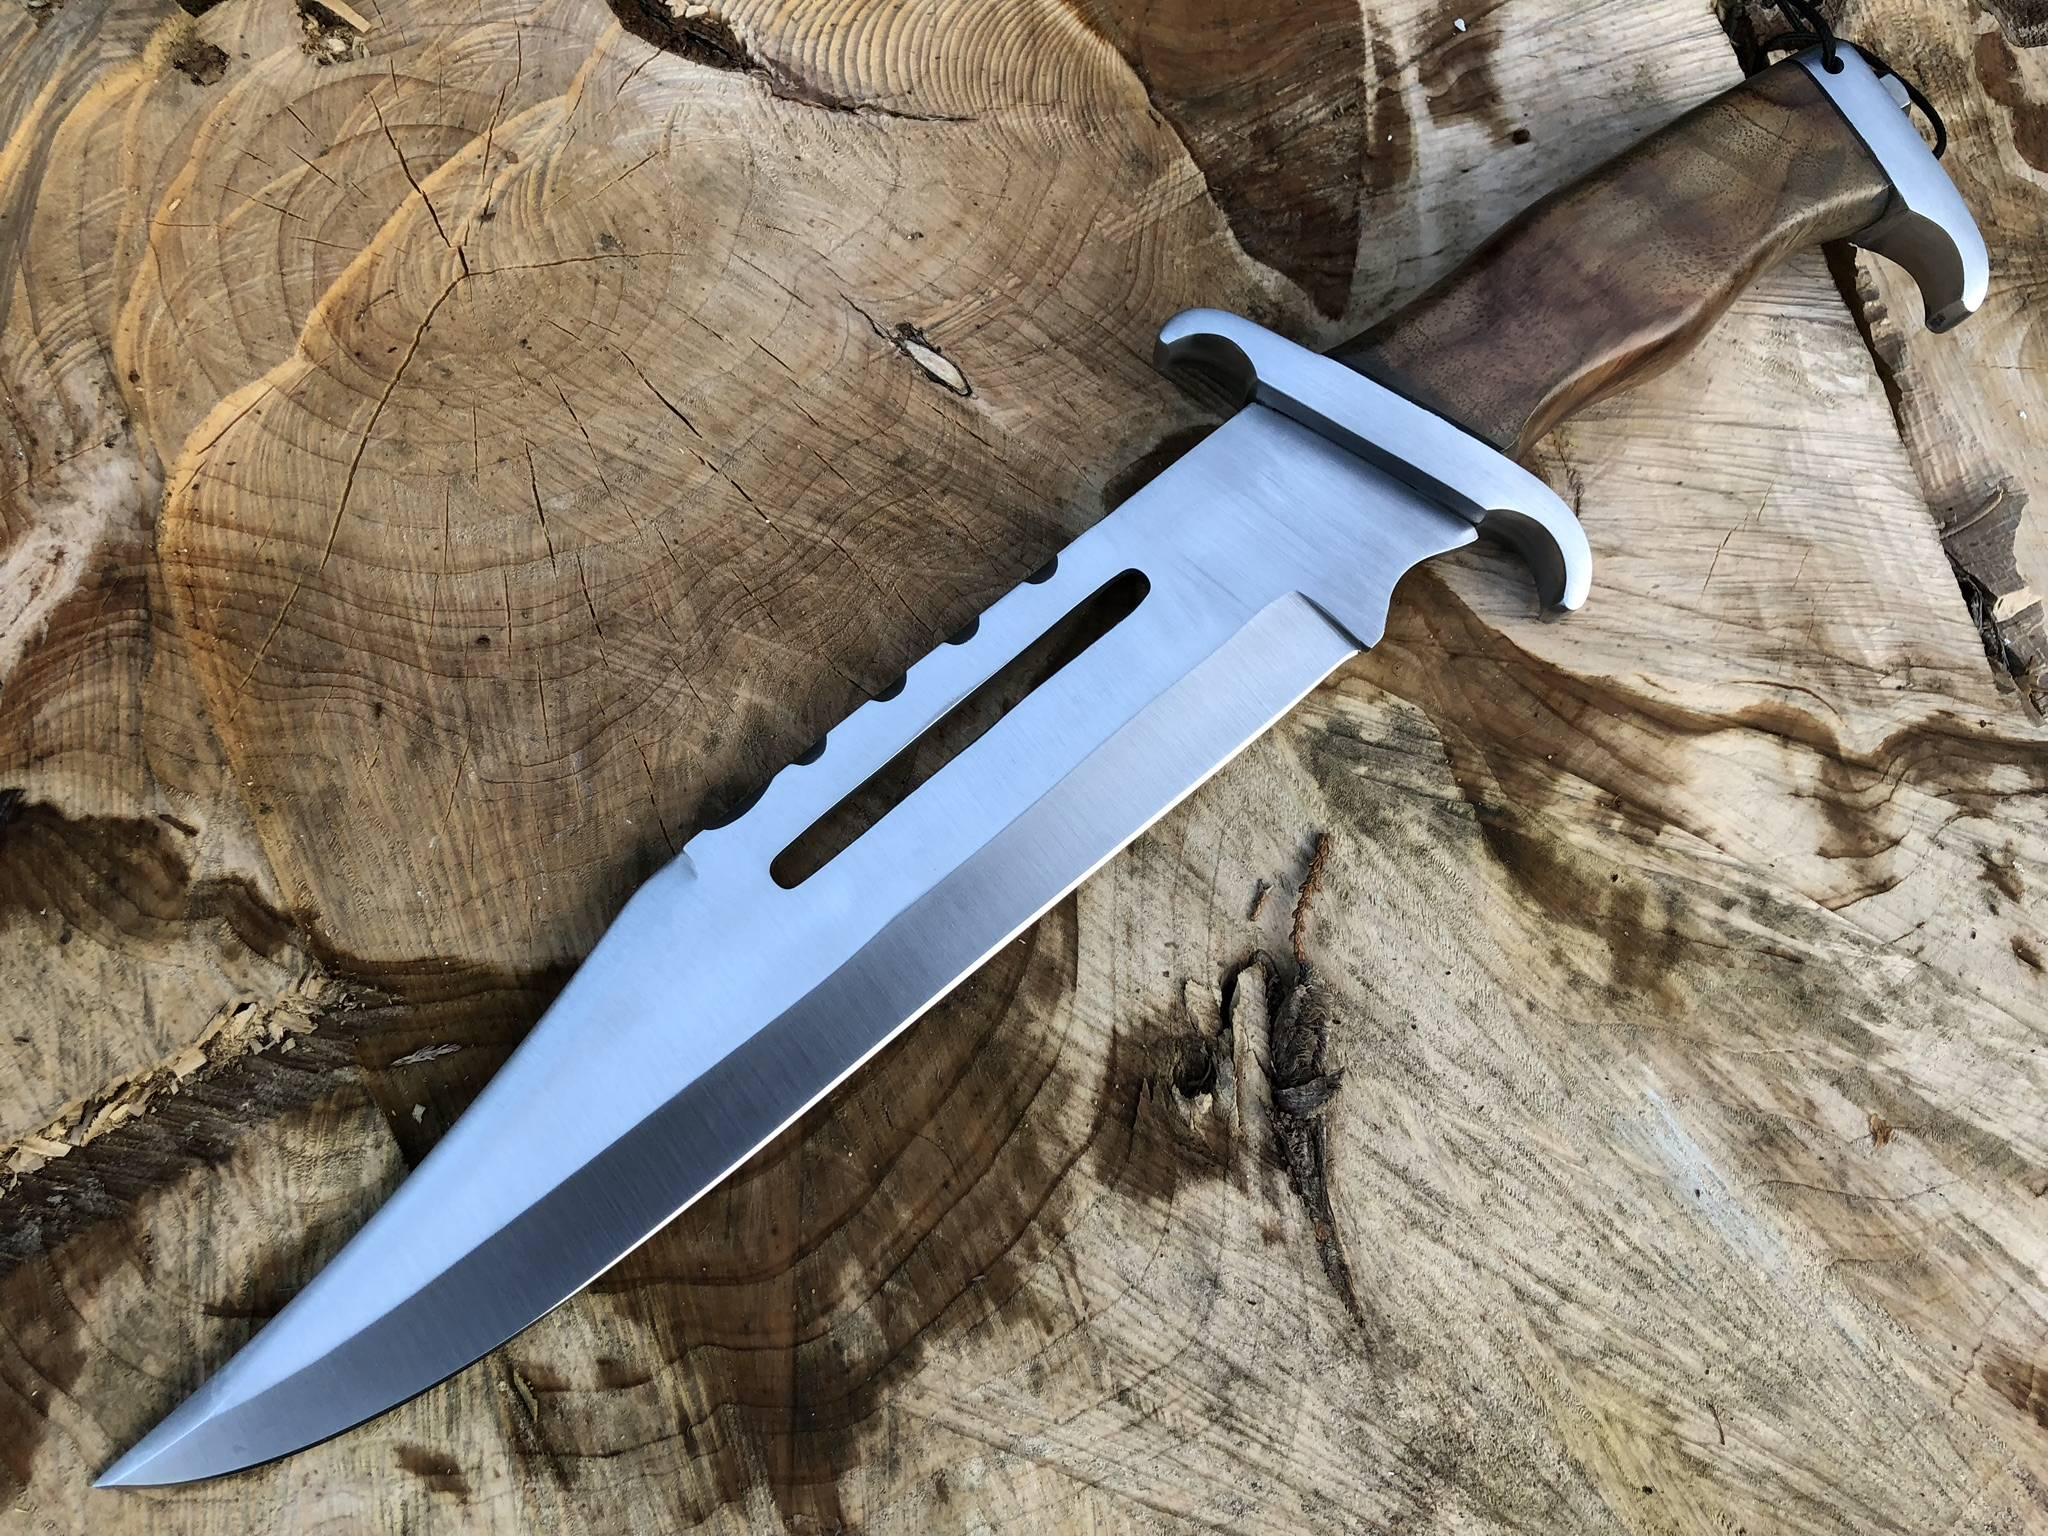
\includegraphics[width=1\linewidth]{figs/knife.jpg}
        \caption{Knife Example}
        \label{fig:first_image}
    \end{minipage}\hfill
    \begin{minipage}{0.48\textwidth}
        \centering
        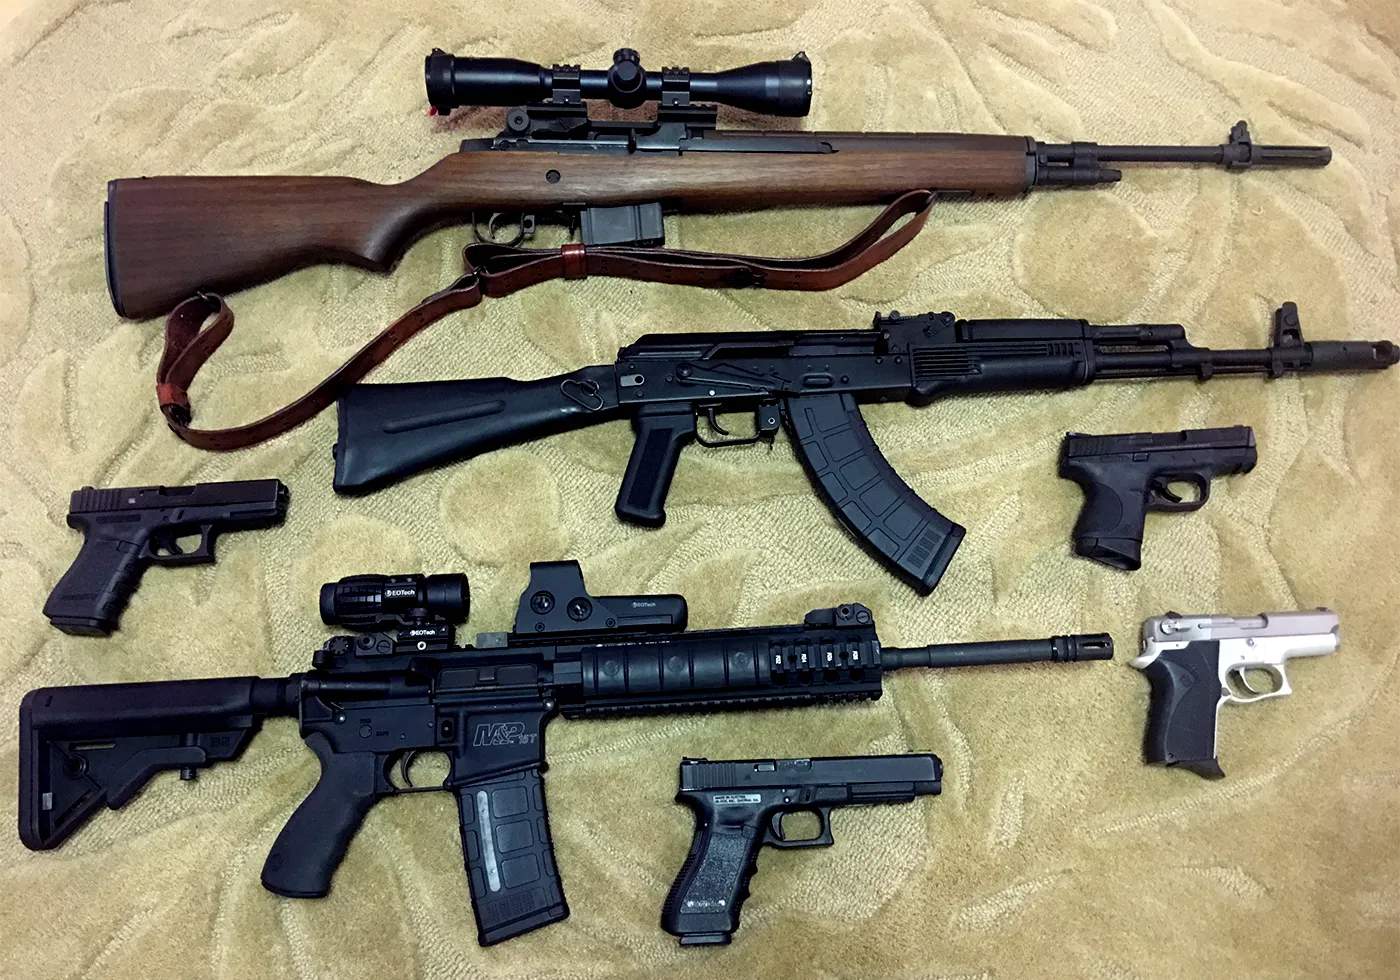
\includegraphics[width=1\linewidth]{figs/firearm.png}
        \caption{Different Firearms Example}
        \label{fig:second_image}
    \end{minipage}
\end{figure}

\subsection{\ac{cctv}}
\ac{cctv} refers to a video surveillance system comprising strategically positioned cameras in various locations. These cameras capture footage, which is then transmitted to monitors for both real-time observation and later playback.

The primary goal of a \ac{cctv} system is to enhance area security through persistent surveillance of key areas. This is highly beneficial for large spaces or sites containing valuable or sensitive items. Besides recording, \ac{cctv} can issue alerts for detected motion, especially during off-hours in vacant business premises. These alerts are crucial for quickly informing authorities about possible security threats.

Additionally, \ac{cctv} systems are not only instrumental in monitoring activities during both operational and non-operational hours but also serve as crucial tools in identifying suspects in criminal activities.

\begin{figure}[h]
    \centering
    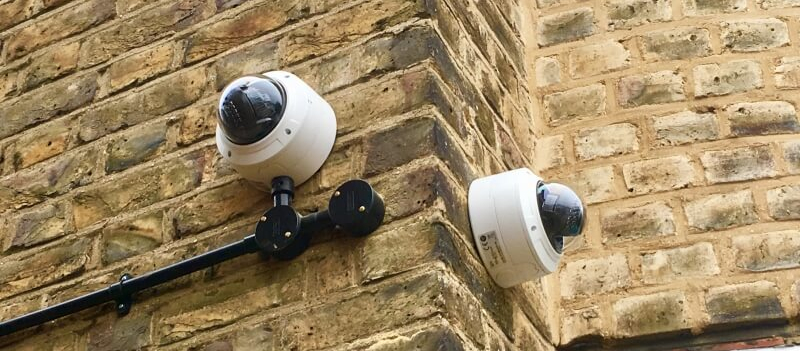
\includegraphics[width=0.45\textwidth]{figs/cctv.jpg}
    \hfill
    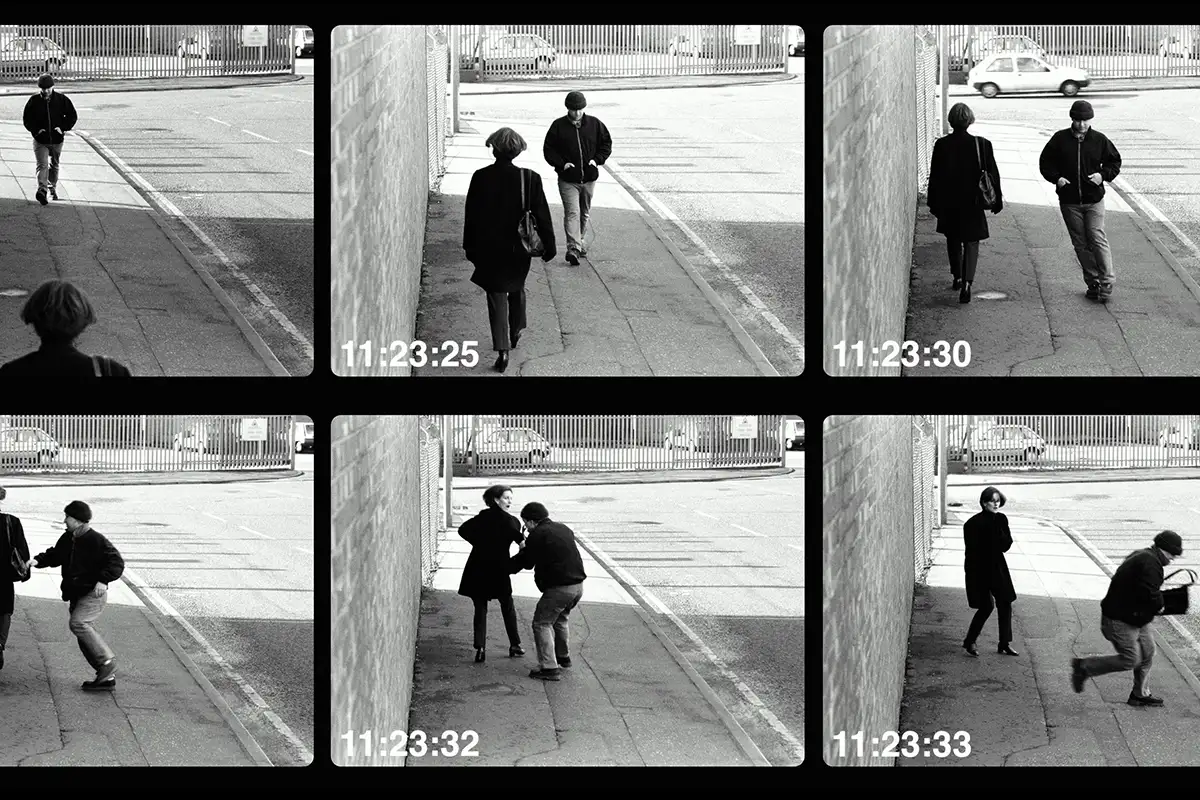
\includegraphics[width=0.45\textwidth]{figs/cctv-footage.png}
    \caption{\ac{cctv} Cameras (Left Image) and \ac{cctv} Footage Samples (Right Image)}
    \label{fig:cctv-and-footage}
\end{figure}

\section{Object Detection}
\subsection{General Concepts}
Object detection stands as a vital component in the realm of computer vision. \selectlanguage{english}\citet{rfc2} describe its goal as "to determine where objects are located in a given image (object localization) and which category each object belongs to (object classification)", undertaking the dual challenge of not only locating an object within the visual frame, creating a bounding box around it, but also determining its category. \selectlanguage{english}\citet{rfc9} further reinforce this stating "Object detection is a fusion of object location and object classification task".

\begin{figure}[h]
    \centering 
    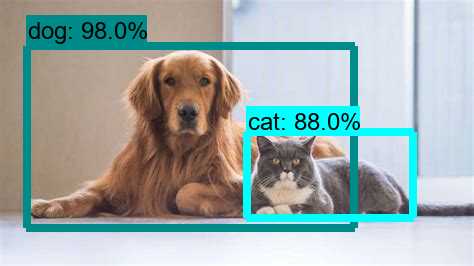
\includegraphics[width=0.5\textwidth]{figs/object-detection.png} 
    \caption{Object Detection Image~\cite{rfc15}}
    \label{fig:object-detection}
\end{figure}

Object detection entails the identification of objects within images and videos. The process of recognizing these objects is fundamentally rooted in the training of object detection models. This crucial training phase involves several key steps:
\begin{itemize}
    \item \textbf{Data Collection}: Gathering a diverse set of images, each showcasing the object in a variety of contexts, including different backgrounds and angles.
    \item \textbf{Labeling}: Annotating each image with labels to show where the object is and confirming its presence
    \item \textbf{Feature Learning}: The neural network learns the object's unique features (like shape, color, texture, patterns) from these labeled images.
    \item \textbf{Generalization}: The ultimate goal of this training is to enable the neural network to not just recognize the object in the training images, but to generalize this knowledge. This allows the model to accurately identify and locate the object in new, unseen images.
\end{itemize} 

The 2014 milestone, Figure \ref{fig:stage-detectors}, marks a pivotal before-and-after in \ac{ai} applications \selectlanguage{english}\cite{rfc22}. Before, the field predominantly utilized traditional methods for tasks like object detection. These methods involved a multi-step process beginning with the selection of regions in images, which was often inefficient and computationally expensive due to the use of techniques like multi-scale sliding windows. Following this, feature extraction methods such as HOG, Haar-like, and SIFT were employed, but these struggled with variability in backgrounds and lighting conditions. The final step, classification, relied on algorithms like Adaboost, but these traditional techniques frequently fell short in terms of accuracy and efficiency \selectlanguage{english}\cite{rfc9}.

After 2014, the landscape of \ac{ai} research underwent a significant transformation with the advent of deep learning-based methods. These new techniques, including \ac{frcnn}, \ac{ssd}, and \ac{yolo}, revolutionized object detection by automatically learning feature representations from data. This shift not only addressed the limitations of the traditional methods, such as high computational costs and inadequate feature representation, but also led to substantial improvements in both the accuracy and efficiency of object detection processes.

\begin{figure}[h]
    \centering 
    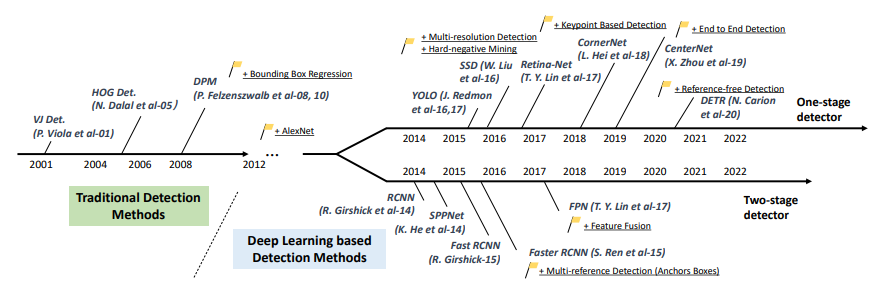
\includegraphics[width=0.97\textwidth]{figs/roadmap-stage.png} 
    \caption{Object Detection Roadmap~\cite{rfc22}}
    \label{fig:stage-detectors}
\end{figure}

There are two primary methodologies, Figure \ref{fig:stage-detectors}, employed for identifying and classifying objects. These methodologies differ significantly in their operational approach and performance characteristics.

Firstly, there is the \textbf{two-stage} detection process. This operate in a sequential two-phase process. The process involves two key steps: "(i) use a Region Proposal Network to generate regions of interests in the first stage and (ii) send the region proposals down the pipeline for object classification and bounding-box regression"\selectlanguage{english}\cite{rfc21}. The two-stage framework ensures high accuracy but at the cost of speed.

Conversely, \textbf{one-stage} detectors treat object detection as a simple regression problem, directly analyzing the image to determine class probabilities and bounding box coordinates. This approach is faster but generally achieves lower accuracy rates compared to two-stage detectors \selectlanguage{english}\cite{rfc23}.

In the field of object detection a variety of metrics are employed to evaluate the performance of detection models. These metrics play a crucial role in both training and testing stages, optimizing classifiers, and measuring their efficiency. 

Precision is calculated as the percentage of correctly identified objects (true positives) among all detections (true and false positives). High precision indicates a low rate of false positives. Recall assesses the model's ability to detect all relevant objects in the dataset. It is the percentage of correctly detected objects (true positives) among all actual objects (sum of true positives and false negatives). High recall implies that the model is effective in identifying most of the relevant objects \selectlanguage{english}\cite{rfc25}.

Following this, accuracy measures the overall correctness of the model, reflecting the proportion of all true results (true positives and true negatives) against the total number of cases.

The \ac{ap} metric integrates precision and recall at different confidence thresholds. It addresses the trade-off between precision and recall, considering detections above a confidence level. \ac{ap} is calculated based on the area under the precision-recall curve \selectlanguage{english}\cite{rfc25}. \ac{map} averages the \ac{ap} across all classes within a database, crucial for assessing multi-class detector performance \selectlanguage{english}\cite{rfc24}. 

F1 score is used to estimate the balance between recall and precision. It is particularly valuable in situations where there is an imbalanced class distribution, as it provides a single metric that combines both precision and recall. Is defined as the harmonic mean\footnote{type of average that gives equal weight to both precision and recall, unlike the arithmetic mean which can be disproportionately influenced by high values of one metric over the other} of precision and recall, \ref{eq:f1score}. 

\begin{equation}
    F1 \text{ score} = 2 \times \frac{\text{Precision} \times \text{Recall}}{\text{Precision} + \text{Recall}}
    \label{eq:f1score}
\end{equation}
    
A high F1 score indicates both high precision and high recall. This metric is particularly useful in the context of binary classifiers on unevenly distributed datasets, where it provides a more balanced view of a model's performance compared to using precision or recall alone \selectlanguage{english}\cite{rfc9}.

\ac{iou} measures the overlap between the predicted \ac{bb} and the ground truth \ac{bb}, Figure \ref{fig:iou}. It's calculated as the ratio of the intersection area to the union area of these BBs. The resulting \ac{iou} value ranges between 0 and 1, with values closer to 1 indicating more accurate detection. "The IoU, based on the Jaccard Index, measures the overlap between the predicted bounding box and the ground-truth bounding box." \selectlanguage{english}\cite{rfc24}.

\begin{figure}[h]
    \centering 
    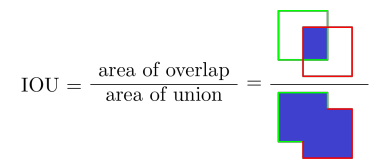
\includegraphics[width=0.5\textwidth]{figs/iou.png} 
    \caption{Intersection over Union \selectlanguage{english}\cite{rfc25}}
    \label{fig:iou}
\end{figure}

\subsection{Algorithms and Techniques Reviews}
This section analyzes current object detection algorithms and methodologies, drawing on a range of studies and innovations from various online repositories and databases. It focuses on selected reviews\footnote{comprehensive overview or evaluation of existing literature on a particular topic} that detail their development, methodologies, outcomes, and contributions to the advancement of object detection. This analysis provides insights into the evolution of object detection techniques from their inception to modern applications.

\selectlanguage{english}\citet{rfc2} delve into the evolution of detection methods, offering a comprehensive review of deep learning-based object detection frameworks. The review starts with a historical overview of deep learning, highlighting the role of \ac{cnn}. The focus then shifts to generic object detection architectures, discussing modifications and strategies to enhance detection performance. Through experimental analyses, various methods for detection tasks are compared, and insightful conclusions are drawn.

\selectlanguage{english}\citet{rfc8} provide a comprehensive review of image processing techniques, emphasizing machine learning applications in visual interpretation. The study begins by highlighting the foundational aspects of computational vision, particularly the significance of array-based media computation in the digital era. It then examines key image processing algorithms, including \ac{ssd}, \ac{frcnn}, and \ac{yolo}, detailing their architecture, methodologies, and distinguishing features. The researchers conduct systematic experiments using datasets like Microsoft COCO~\cite{rfc16}, comparing these algorithms to elucidate their respective strengths and limitations.

\selectlanguage{english}\citet{rfc9} emphasize the intricacies of computer vision in their review, highlighting the significant impact of \ac{dcnns}. Their study spans various applications, from video processing to speech recognition, with a particular focus on object detection's importance in areas like transportation and security. They detail crucial evaluation metrics, especially Average Precision (AP), for assessing detection effectiveness. Notably, they mark the pivotal shift to deep learning techniques post-2014, analyzing frameworks like \ac{ssd} and \ac{yolo}. By comparing these newer methods with traditional ones and evaluating their performance on datasets like PASCAL VOC~\cite{rfc27} and MS COCO~\cite{rfc16}, they offer insights into the dynamic field of object detection.

\selectlanguage{english}\citet{rfc10} present an in-depth review of \ac{dl}, focusing on its essential concepts, \ac{cnn} architectures, challenges, and varied applications. The paper initially recognizes DL's increasing prominence in machine learning, often hailed as the 'Gold Standard.' Emphasizing DL's efficiency in processing large datasets, surpassing traditional methods, the authors delve into detailed \ac{cnn} architectures and their operational principles. They also explore both computational and conceptual challenges in DL. The review further highlights the diverse applications of DL, showcasing its often superior, sometimes human-competitive, performance.

\section{Related Work}
In the quest for enhancing weapon detection capabilities in CCTV systems, a range of significant studies have emerged, each contributing distinctive methodologies, techniques, and insights. 

This section is dedicated to presenting a comprehensive overview of these contributions, systematically organized into focused areas: research methodologies, an in-depth comparative analysis of weapon detection technologies, a thorough exploration of datasets pertinent to this field, and a review of the various architectural approaches employed in weapon detection systems.

\subsection{Research Method}
This section presents a comprehensive review of critical research in the field of weapon detection. The review is structured into four key areas: \ac{cctv} setup and installation, insights from other researchers' literature, pertinent datasets, and prevalent system architectures. Due to the wide range and variety of articles from different fields, a careful selection method was used. The search, conducted on Scopus, ResearchGate, and arXiv, focused on keywords like "deep," "learning," "real," "time," "weapon," and "detection." This search initially produced a large number of articles. A detailed and strict selection process was then applied to choose the most relevant articles that significantly relate to the main theme.

\subsection{\ac{cctv} System Setup and Configuration}
Ensuring the effectiveness of a \ac{cctv} security system requires careful consideration of several key factors. Analyzing the environmental context of the camera location is critical. It involves understanding the specific crime dynamics of the area and strategically positioning the cameras to cover high-risk zones. The line-of-sight for each camera also demands attention. To ensure clear visibility, it's important to minimize obstructions such as immovable objects and foliage. Regular maintenance is crucial to clear any new obstructions that may arise. Regular maintenance to clear any new obstructions is also crucial. 

The design of the cameras significantly influences their ability to prevent crime. Semi-covert 'dome' cameras, Figure \ref{fig:semi-dome}, are often more effective in discouraging criminal activities compared to overt cameras, Figure \ref{fig:covert}, making them a preferable choice in many scenarios. An effective \ac{cctv} system is not just about installation but also involves active monitoring and prompt enforcement actions \selectlanguage{english}\cite{rfc4}.
\begin{figure}[h]
    \centering

    % Image 1
    \begin{minipage}{0.3\textwidth}
        \centering
        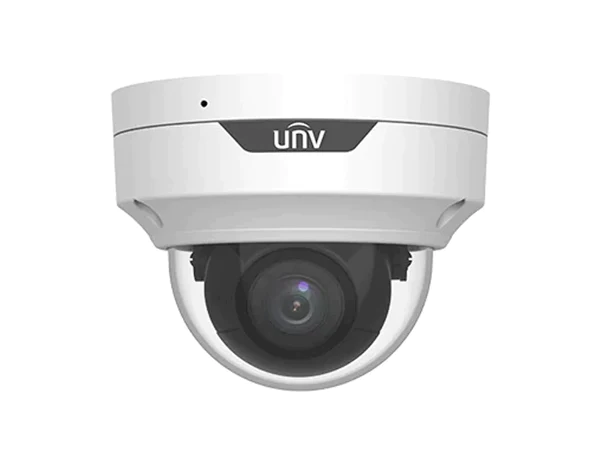
\includegraphics[width=\textwidth]{figs/semi-dome.png} % Include the image
        \caption{Semi-covert dome camera}
        \label{fig:semi-dome}
    \end{minipage}
    \hspace{2cm}
    % Image 2
    \begin{minipage}{0.32\textwidth}
        \centering
        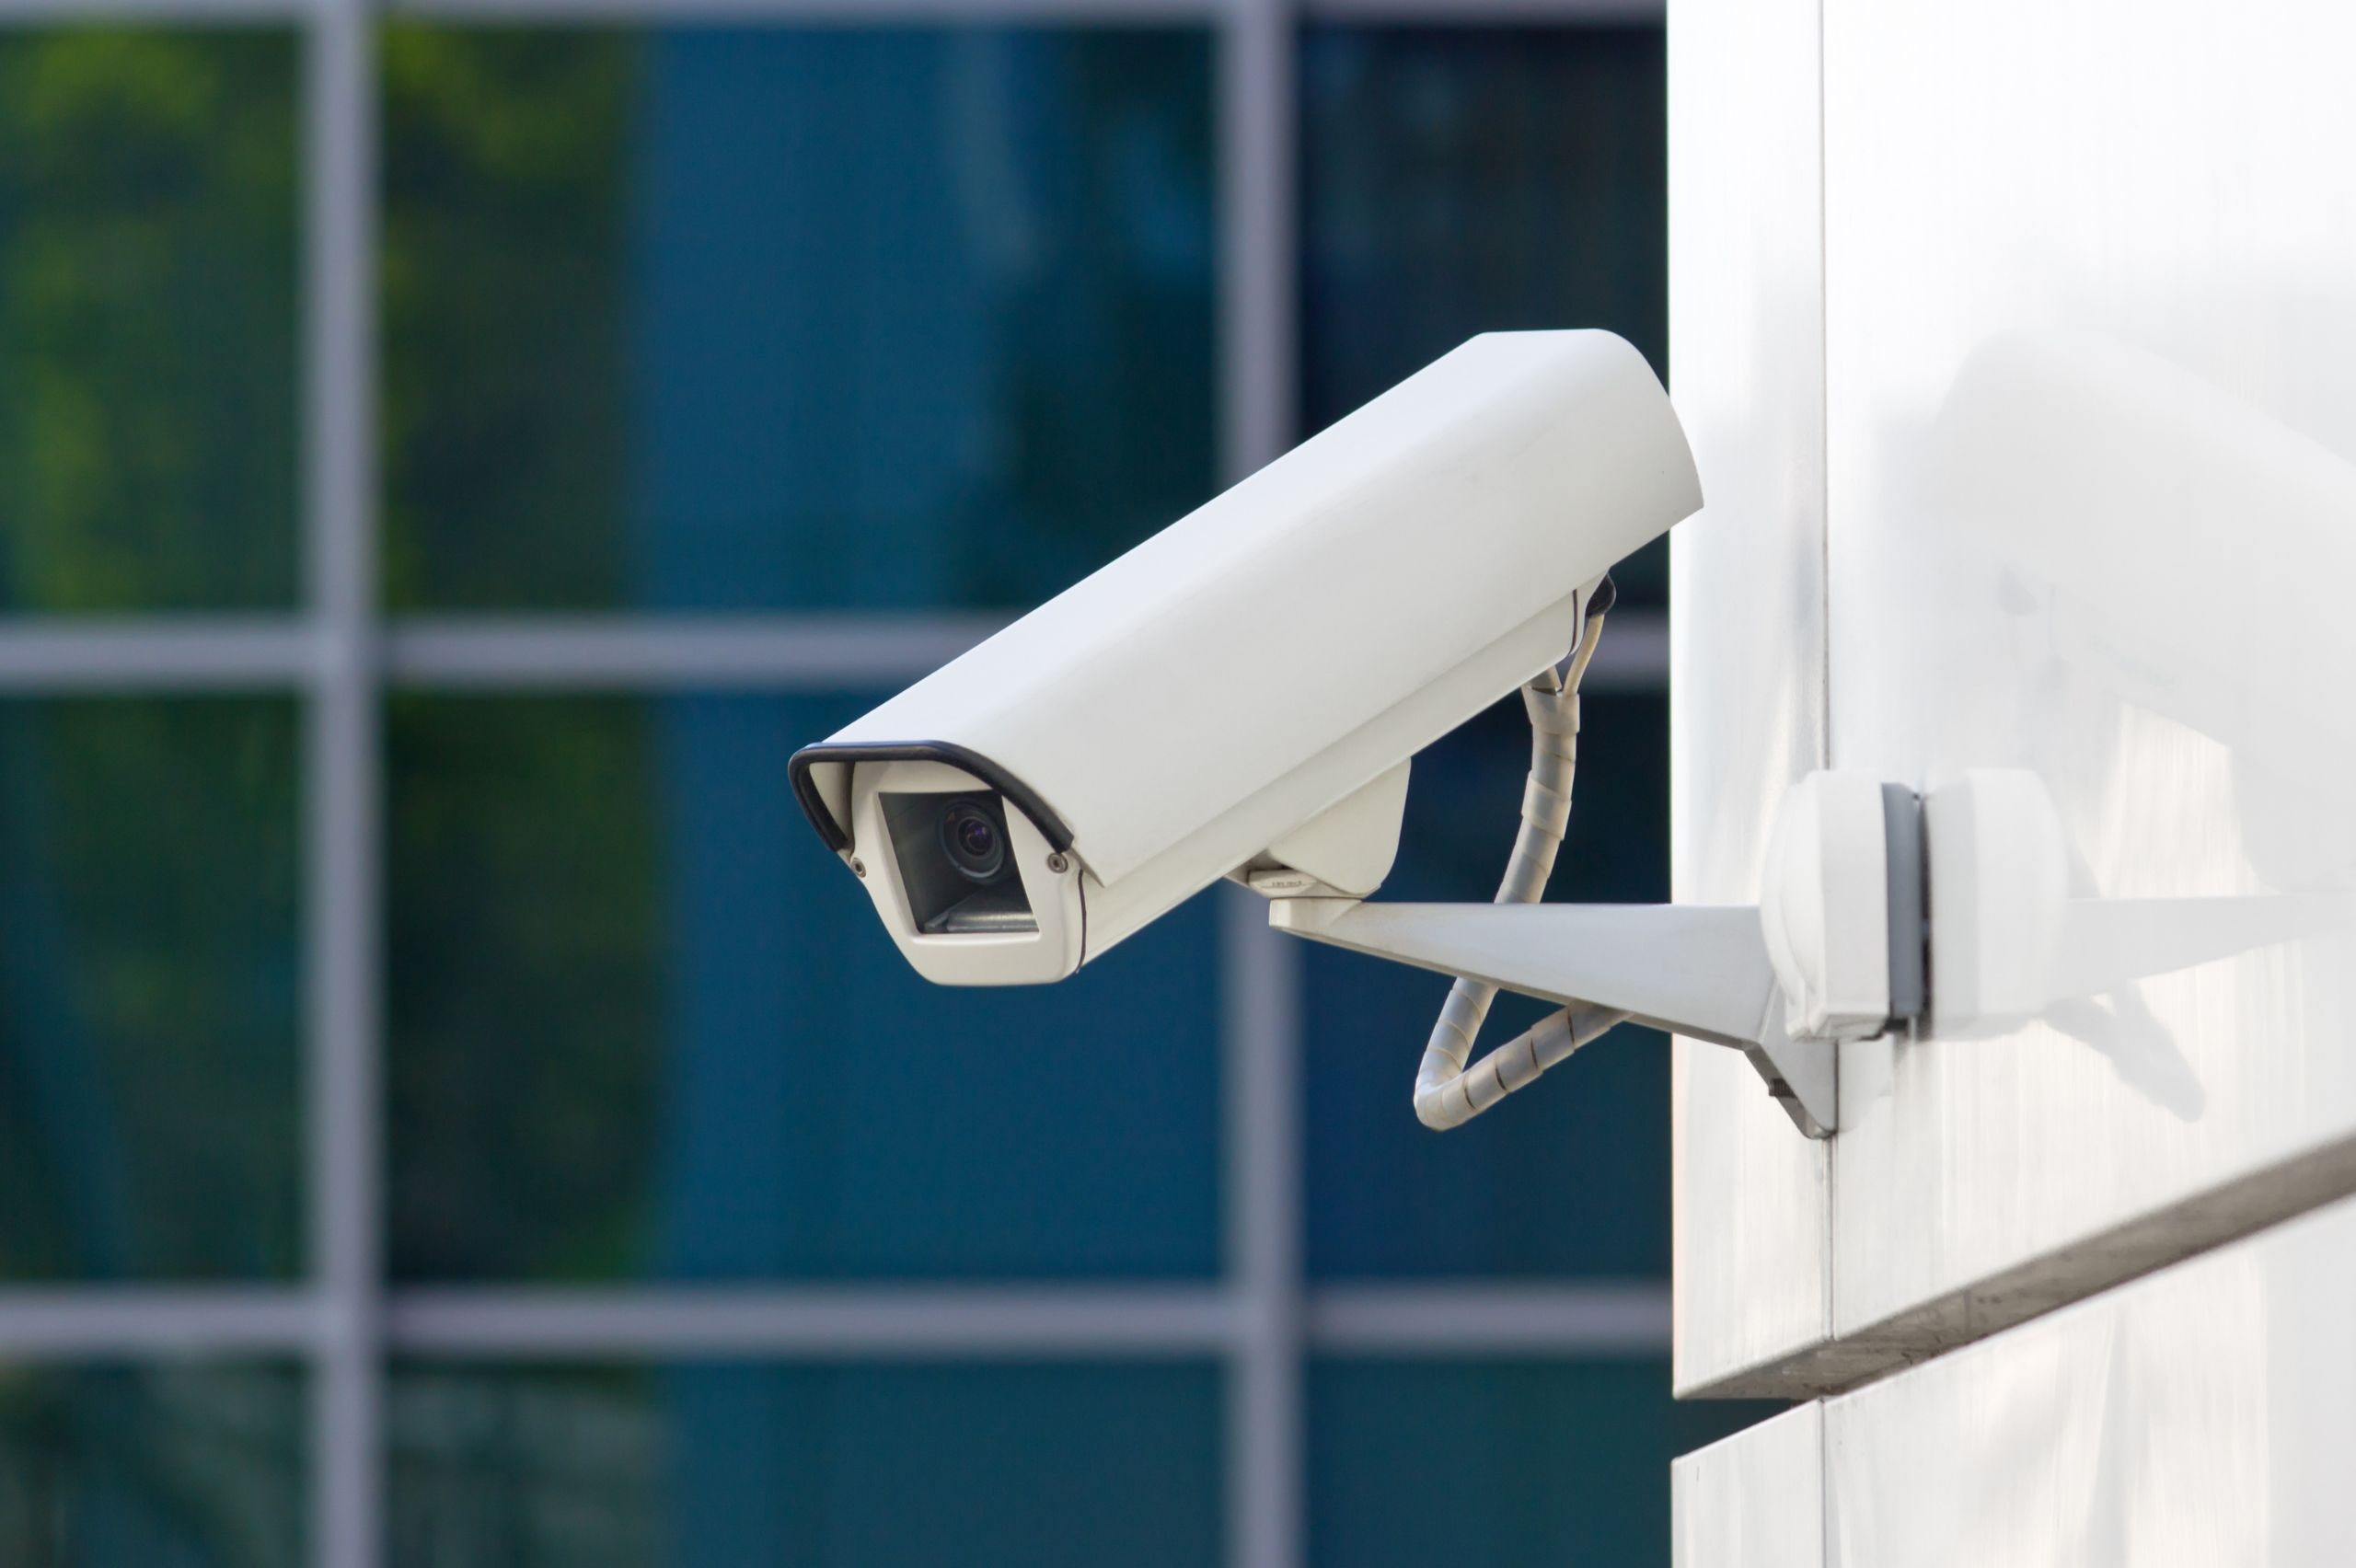
\includegraphics[width=\textwidth]{figs/overt2.jpg} % Include the image
        \caption{Covert cameras}
        \label{fig:covert}
    \end{minipage}
\end{figure}

\selectlanguage{english}\citet{rfc42} identified a spectrum of problems in control room environments, specifically in the management and operation of \ac{cctv} systems. A critical aspect highlighted is the poor configuration of technology in these environments. This includes improperly positioned cameras in low-crime zones or areas with blind spots, and the adverse effects of weather on analog signals. Additionally, outdated or malfunctioning equipment, like broken camera controllers, further impairs surveillance effectiveness. The quality of video recordings was another area of significant concern. Many control rooms recorded footage at low resolutions, rendering it ineffective for detailed analyses or criminal investigations.

\citet{rfc46} proposed a model which delineates a community's surveillance blueprint, marking the prime locations for \ac{cctv} installation. 
\begin{itemize}
    \item Red dots represent primary entry and exit points, ensuring close monitoring of individual movements through these areas;
    \item Black dots are placed at street intersections and corners, providing broad surveillance coverage;
\end{itemize}

In this model, cameras positioned at red dots 
would be pivotal for controlling access points, while those at black dots would enable panoramic monitoring 
of the area, essential for observing multiple streets and deterring potential criminal activity. 

\begin{figure}[h]
    \centering 
    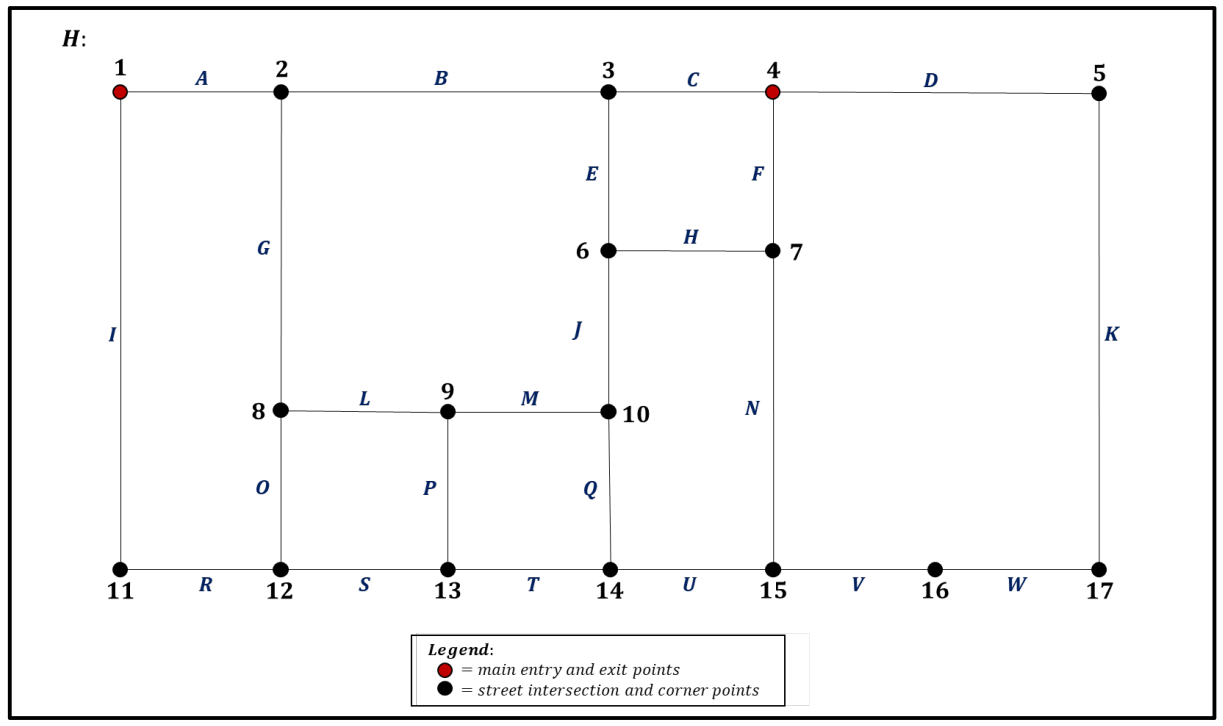
\includegraphics[width=0.75\textwidth]{figs/cctv-positions.png} 
    \caption{Labeled Graph H (Simple Graph Representation of District 5) \selectlanguage{english}\cite{rfc46}}
    \label{fig:cctv-positions}
\end{figure}


\subsection{Analysis of Existing Datasets in Weapon Detection Research}
In real-time weapon detection, using datasets that mimic real-world situations is crucial.

In~\citet{rfc3} study, the dataset comprises three distinct classes: short guns, long guns, and knives - Figure \ref{fig:rehman-dataset}. This dataset is gathered from a variety of platforms, including surveillance videos from YouTube, simulations of firearms and knives created within the Unity framework, and images of pistols, revolvers, and knives from the Open Images Dataset as well as Kaggle. For video, a set of individual frames was extracted and manually labeled using the LabelImg Python utility. To enhance the model's training performance, data augmentation techniques were employed.

\begin{figure}[h]
    \centering 
    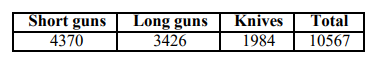
\includegraphics[width=0.45\textwidth]{figs/rheman-dataset.png} 
    \caption{Dataset images classes number~\cite{rfc3} }
    \label{fig:rehman-dataset}
\end{figure}

\selectlanguage{english}\citet{rfc4} developed datasets for real-time weapon detection, focusing on pistols in various settings. Data was sourced from the internet, YouTube, GitHub, research groups, and the Internet Movie Firearm Database \selectlanguage{english}\cite{rfc28}, leading to three datasets categorized into 'Pistol' and 'Not-Pistol' classes, Figure \ref{fig:bathi-dataset}. The 'Pistol' class contained handheld weapons like pistols and revolvers, while 'Not-Pistol' included objects often confused with weapons, like wallets and cell phones. The researchers standardized image size and resolution during data preparation, applied mean normalization, and used data augmentation to enhance the dataset, aiding the model's generalization capabilities.
\begin{figure}[h]
    \centering 
    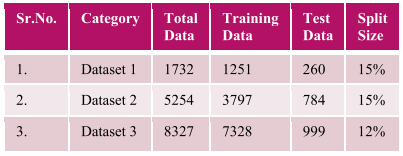
\includegraphics[width=0.45\textwidth]{figs/bathi-dataset.png} 
    \caption{Datasets created by~\cite{rfc4}}
    \label{fig:bathi-dataset}
\end{figure}

\selectlanguage{english}\citet{rfc5} used Google Collab \selectlanguage{english}\cite{rfc26} to train models on 1496 images using \ac{yolo}v3 and \ac{yolo}v5 with pre-trained COCO dataset weights \selectlanguage{english}\cite{rfc16}. The images were divided into 1200 for training and 296 for validation and testing (148 each). Training lasted 40 epochs, taking about 120 minutes, with images sized at 416x416 pixels. Both models, within the PyTorch framework, utilized a COCO pre-trained backbone feature extraction network, which was fine-tuned during training to better represent handguns.

\selectlanguage{english}\citet{rfc6} used a comprehensive dataset consisting of 10,014 distinct weapon images to train and evaluate the model's accuracy. These images were categorized into three primary object types: knives, with a total of 3,641 images; long guns, comprising 2,497 images; and small guns, which included 3,876 images. The dataset was strategically divided, allocating 80\% of the images (8,011 images) for training and the remaining 20\% (2,003 images) for testing. Each image used had a resolution of 240 x 240 pixels, and during the training phase, they were processed in batches of 32.

\selectlanguage{english}\citet{rfc7} and Moran et al. \selectlanguage{english}\citet{rfc18} both utilized the DaSCI Weapon Dataset \cite{rfc29} for weapon detection research, with \selectlanguage{english}\citet{rfc7} focusing on differentiating weapons from ordinary objects and training their system on 91 weapons. Additionally, employed the CAVIAR Dataset \cite{rfc30} for Suspicious Behavior Prediction, using its video clips of six human actions, annotated in XML, to classify actions as suspicious or not. They parsed XML files to align annotations with video frames for analysis. \selectlanguage{english}\citet{rfc18} used the DaSCI Dataset \cite{rfc29} for knife detection, comprising 2,078 images, primarily from the internet and YouTube. They also utilized the MS COCO 2017 Dataset \cite{rfc16}, a larger dataset with 330,000 images in 80 classes, including 4,326 images labeled under the 'knife' class.

\selectlanguage{english}\citet{rfc17} faced challenges in gathering a comprehensive weapon dataset, particularly for knife and screwdriver images, due to the lack of labeled datasets suitable for classifier training. To overcome this, they used web scraping to gather images from websites and GitHub. These images were manually labeled with tools like LabelImg and Roboflow, and standardized to a 416 x 416 resolution. Their final dataset contained about 6,000 images, with 2,000 each of pistols, knives, and screwdrivers. For training and testing their models, they divided the images in an 80:20 ratio.

\selectlanguage{english}\citet{rfc19} installed a Raspberry Pi B+ with a camera 1.8m high to capture images of consenting students with handgun replicas at a lab entrance. They initially collected 14k images at 1920x1080 resolution, which were expanded to 28k after data augmentation. A challenge in their study was the small size of the guns in the images, posing a risk of misclassification.

\selectlanguage{english}\citet{rfc20} used the ARMAS Weapon Detection Dataset and IMFDB Weapon Detection System \cite{rfc28} for firearm-related crime image collection. The datasets included 3000 and 4940 images of pistols and rifles, respectively. These images underwent preprocessing to fit object detection standards and were split into training and testing sets in an 80:20 ratio.

\subsection{Review of Architectural Approaches in Weapon Detection}
The evolution of real-time weapon detection systems has been significantly influenced by diverse architectural approaches proposed by various researchers. This section delves into a brief analysis of some of these architectures.

\selectlanguage{english}\citet{rfc44} system's operation begins with a Raspberry Pi Camera, which serves as the image capture device, feeding live images into the processing unit, a Raspberry Pi. Once the images are pre-processed, they are fed into a pre-trained Deep Neural Network (DNN) weapon detection model. Upon successful detection of a weapon, the system activates an alert mechanism. Finally, the system sends a notification along with the images of the detected weapon to a smartphone.

\begin{figure}[h]
    \centering 
    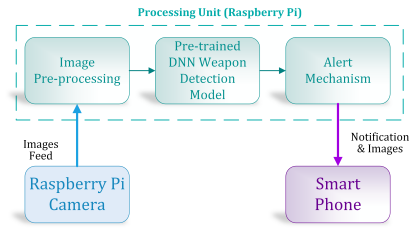
\includegraphics[width=0.36\textwidth]{figs/uob-architecture.png} 
    \caption{\selectlanguage{english}\citet{rfc44} System Diagram}
    \label{fig:uob-architecture}
\end{figure}

One of the standout features of \selectlanguage{english}\citet{rfc6} architecture, Figure \ref{fig:gawade-architecture}, is its integration of an alarm system that activates upon successful weapon detection, thereby ensuring immediate alert to security personnel. This aspect of the model not only enhances its practical application but also significantly contributes to the safety and security in public spaces like malls, airports, and railway stations.
\begin{figure}[h]
    \centering 
    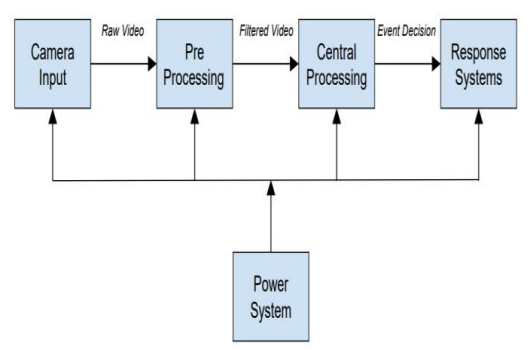
\includegraphics[width=0.4\textwidth]{figs/Gawade-architecture.png} 
    \caption{\selectlanguage{english}\citet{rfc6} Architecure Diagram}
    \label{fig:gawade-architecture}
\end{figure}

\selectlanguage{english}\citet{rfc17} architecture relies on the \ac{yolo}v8 algorithm. The process begins with collecting a large set of images that will be used to teach the detection model what various weapons look like. Each image is then labeled to identify where the weapons are. Once the images are labeled, they are processed to ensure they're in the right format for the model to learn from them effectively. Next, the images are used to train the \ac{yolo}v8 object detection model. Finally, if the system assesses the situation as a medium or high threat, it sends an alert to security guards. This alert includes the image where the weapon was detected and details about the threat level.

The \citet{rfc7} system initiates surveillance and processes the input from two sources: a live webcam and test videos, Figure \ref{fig:shenoy-architecture}. For the live webcam input, the system employs face detection technology to locate human faces within the video frames. If a face is detected, the next step is face recognition, where the system compares the detected face against a database of known criminal records. Simultaneously, the system also runs object detection algorithms to identify potential weapons in the scene. The input from test videos, on the other hand, is fed into a CNN-GRU model. When either the live feed or the test video analysis results in the identification of a criminal, the detection of a weapon or suspicious behavior, the system converges these findings to determine if there's a crime happening. If a crime is detected, the system generates an alert and sends a notification to the concerned authorities.

\begin{figure}[h]
    \centering 
    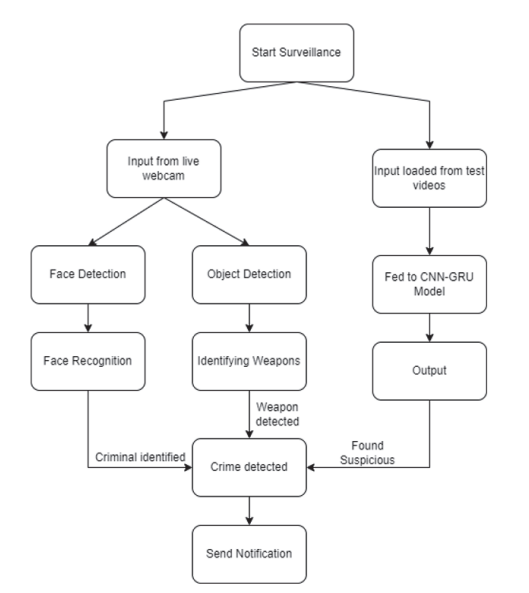
\includegraphics[width=0.6\textwidth]{figs/shenoy-architecture.png} 
    \caption{\citet{rfc7} System Architecture}
    \label{fig:shenoy-architecture}
\end{figure}

\subsection{Comparative Analysis of Weapon Detection Technologies}
\selectlanguage{english}\citet{rfc3} point out the concern of incidents involving firearms and knives due to insufficient security checks. Despite \ac{cctv}s have become prevalent, their constant surveillance demands often surpass human monitoring capabilities. The paper introduces an automated weapon detection system, which employs the \ac{yolo}v5 deep learning model, adapted to a carefully selected dataset. The obtained results achieved a F1 score of 0.95 when applied to \ac{cctv} footage.

\selectlanguage{english}\citet{rfc4} emphasize the importance of security for economic growth and attracting investors and tourists. The study addresses the difficulty of detecting weapons in real-time, considering problems like different angles, blocked views, and hidden weapons. A dataset was adapted by the researchers from diverse sources, including original photos, online repositories, and even film databases. Their exploration spanned several algorithms, like VGG16, Inception variants, and \ac{yolo} iterations. Through rigorous testing prioritizing precision and recall over mere accuracy, \ac{yolo}v4 emerged as the frontrunner, achieving a F1-score of 0.91 and a mean average precision of 0.92. To illustrate the methodology behind the advanced surveillance techniques discussed, Figure \ref{fig:bhatti-chart} provides a schematic overview of the relationship between object recognition, including classification and localization, and object detection.

\begin{figure}[ht]
    \centering 
    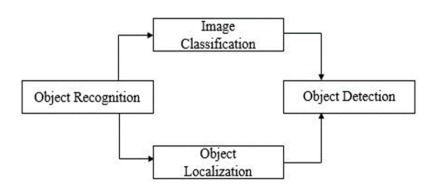
\includegraphics[width=0.43\textwidth]{figs/bhatti-chart.png} 
    \caption{Object recognition to detection hierarchy \cite{rfc4}}
    \label{fig:bhatti-chart}
\end{figure}

In their study, \selectlanguage{english}\citet{rfc5}, address the challenge of detecting concealed weapons in public spaces, despite widespread \ac{cctv} surveillance. They point out the limitations of human monitoring in effectively analyzing extensive footage. To overcome this, they develop an enhanced weapon detection system using the \ac{yolo}v5 deep learning framework, specifically trained on a dataset of 1496 images. This system excels in identifying handguns in various conditions, achieving a \ac{map} of 0.92. Additionally, their comparative analysis with \ac{yolo}v3, as shown in Figure \ref{fig:performance-Thangaraj}, indicates that \ac{yolo}v5 not only improves accuracy in handgun detection but also operates faster and with lower computational demands.

\begin{figure}[h]
    \centering 
    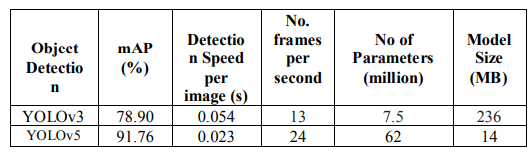
\includegraphics[width=0.55\textwidth]{figs/performance-Thangaraj.png} 
    \caption{Models Performance Comparison \selectlanguage{english}\cite{rfc5}}
    \label{fig:performance-Thangaraj}
\end{figure}

\selectlanguage{english}\citet{rfc18} refers in smart cities context the need for a advanced surveillance applied to urban security. The authors present an approach, combining super-resolution techniques with the \ac{yolo}v4 deep neural network, to detect knives in complex images, a task made difficult by variables like shape, size, and lighting.

\selectlanguage{english}\citet{rfc17}, address the challenge of escalating urban crimes involving firearms and sharp objects in their study. They note the inadequacy of manual monitoring of the extensive data generated by omnipresent \ac{cctv}s in modern cities. To bridge this gap, they have innovated using the \ac{yolo}v8 deep learning framework, tailored to a specialized dataset including images of pistols, knives, and screwdrivers. The system achieved 0.93 accuracy rate on \ac{cctv} footage.

In the security system presented by \citet{rfc19}, a key component of the image processing workflow involves the pre-processing of \ac{cctv} feed images to enhance the performance of the deep learning model, Figure \ref{fig:al-mousa-flow}. The system operates by periodically capturing images from \ac{cctv} feeds and analyzing them with a \ac{cnn}, enabling swift identification of potential threats. A distinctive feature of this system is the immediate notification of security personnel via a mobile app, including an image of the detected threat. The system achieves an accuracy rate of 0.92 and can detect threats within 1.6 seconds.

\begin{figure}[h]
    \centering 
    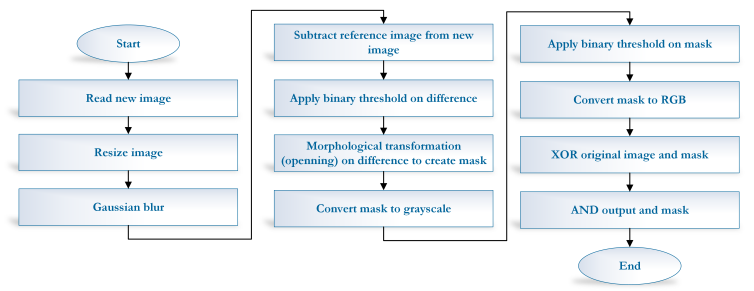
\includegraphics[width=0.65\textwidth]{figs/al-mousa-flowchart.png} 
    \caption{\selectlanguage{english}\citet{rfc19} image pre-processing flowchart}
    \label{fig:al-mousa-flow}
\end{figure}

\selectlanguage{english}\citet{rfc6} research tackles the increasingly alarming scenario of weapon-related threats in crowded public spaces like banks, airports, and railway stations. Recognizing that while the deployment of \ac{cctv} cameras has seen a global surge, the sheer volume of footage can overwhelm human operators. This paper introduces a weapon detection system that uses the power of deep learning, specifically through the use of \ac{cnn}. Trained on a dataset of 10014 images, the model adeptly identifies knives, small guns, and long guns, achieving an accuracy rate of approximately 0.85.

\selectlanguage{english}\citet{rfc20} address the limitations of \ac{cctv} systems, particularly their dependence on manual monitoring by police personnel, by introducing an automated weapon detection system, Figure \ref{fig:hnoohom-system}. Utilizing two public datasets, ARMAS and IMFDB \cite{rfc28}, their research tests various object detection techniques, including \ac{ssd} MobileNet-V1, EfficientDet-D0, and \ac{frcnn} Inception Resnet-V2. The study highlights the effectiveness of \ac{frcnn} Inception V2 with the ARMAS dataset, achieving a \ac{map} of 0.540, and \ac{ap} scores of 0.793 at 0.5 \ac{iou} and 0.627 at 0.75 IoU.
\begin{figure}[h]
    \centering 
    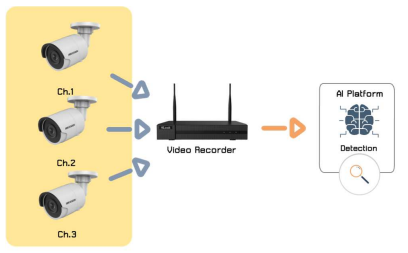
\includegraphics[width=0.37\textwidth]{figs/hnoohom-system.png} 
    \caption{\selectlanguage{english}\citet{rfc20} weapon detection process}
    \label{fig:hnoohom-system}
\end{figure}

\selectlanguage{english}\citet{rfc7} emphasize the alarming rise in criminal activities in urban spaces, despite the ubiquity of \ac{cctv} systems in public areas. Recognizing the limitations of human supervision for these vast surveillance networks, they introduce an intelligent crime detection mechanism. Utilizing the \ac{ssd} Mobilenet architecture fine-tuned on the DaSCI Weapon Dataset \cite{rfc29}, their solution identifies a broad spectrum of weapons, yielding an accuracy rate of 0.81. Moreover, with the integration of the GRU-based behavior analysis model, the system achieved an accuracy of 0.96 in detecting suspicious actions.

Table \ref{models-results} provides a comparative summary of the weapon detection models used by the authors. \ac{yolo} models, particularly \ac{yolo}v5, demonstrate high performance with an F1 score up to 0.95, indicating strong precision and recall. The table also shows that while traditional \ac{cnn} models are effective, with accuracy scores around 0.92, are generally outperformed by the \ac{yolo} series. \ac{frcnn} and \ac{ssd} models show varied results with accuracies ranging from 0.81 to 0.85 and mAP scores as low as 0.54, suggesting they may be less consistent across different datasets. Overall, newer \ac{yolo} models seem to offer a good balance of accuracy and efficiency for object detection tasks.

\begin{table}[ht]
    \centering
    \begin{tabular}{|l|l|l|}
    \hline
    \textbf{Authors} & \textbf{Model} & \textbf{Results} \\ \hline
    \selectlanguage{english}\citet{rfc3} & Yolov5 & F1 Score 0.95 \\ \hline
    \selectlanguage{english}\citet{rfc4} & Yolov4 & F1 Score 0.91, mAP 0.92 \\ \hline
    \selectlanguage{english}\citet{rfc5} & Yolov3, Yolov5 & mAP 0.92 \\ \hline
    \selectlanguage{english}\citet{rfc18} & Yolov4 & - \\ \hline
    \selectlanguage{english}\citet{rfc17} & Yolov8 & Accuracy 0.93 \\ \hline
    \selectlanguage{english}\citet{rfc19} & CNN & Accuracy 0.92 \\ \hline
    \selectlanguage{english}\citet{rfc6} & CNN & Accuracy 0.85 \\ \hline
    \selectlanguage{english}\citet{rfc20} & Faster R-CNN & mAP 0.54, AP 0.79 (0.5 IoU), AP 0.63 (0.75 IoU)  \\ \hline
    \selectlanguage{english}\citet{rfc7} & SSD & Accuracy 0.81 \\
    \hline
    \end{tabular}
    \caption{Authors models and results}
    \label{models-results}
\end{table}

Figure \ref{fig:models-distribution} presents the distribution of different models utilized in previous weapon detection studies, with YOLO models being the predominant choice at 55.6\%, featured in over half of the articles. 

Meanwhile, Figure \ref{fig:metrics-distribution} displays the evaluation metrics that researchers selected for assessing weapon detection models. The Accuracy Rate is the leading metric, employed in 41.7\% of the studies, followed by the F1 Score, which is used in 33.3\% of the cases. The Mean Average Precision (mAP) and Intersection over Union (IoU) metrics are less commonly used, at 16.7\% and 8.3\% respectively.
\begin{figure}[h]
    \centering

    % Image 1
    \begin{minipage}{0.4\textwidth}
        \centering
        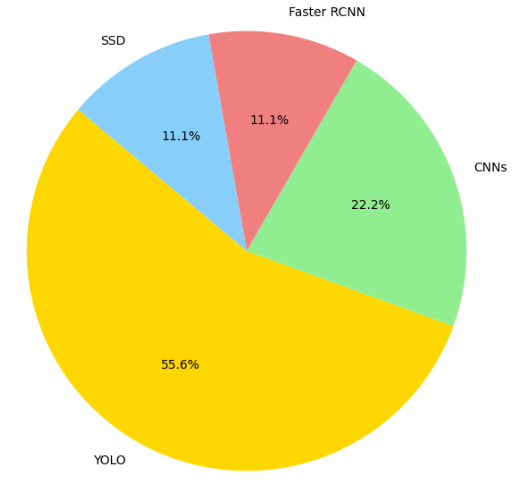
\includegraphics[width=\textwidth]{figs/models-distribution.png} % Include the image
        \caption{Distribution of models used in studies}
        \label{fig:models-distribution}
    \end{minipage}
    \hfill
    % Image 2
    \begin{minipage}{0.5\textwidth}
        \centering
        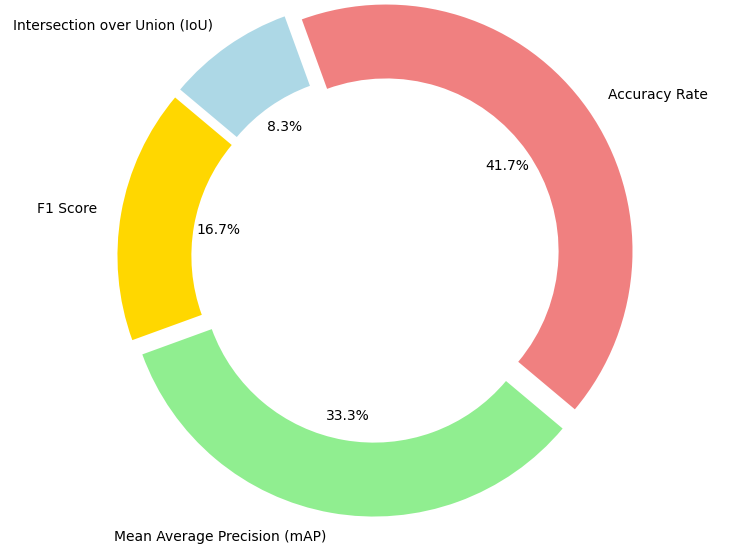
\includegraphics[width=\textwidth]{figs/metrics-distribution.png} % Include the image
        \caption{Distribution of metrics used in studies}
        \label{fig:metrics-distribution}
    \end{minipage}

\end{figure}